\documentclass[output=paper]{langscibook} 
\ChapterDOI{10.5281/zenodo.8269224}

\title[Introduction]{Introduction: Bridging the gap between individual interactions and areal patterns}

\author{Rik van Gijn\affiliation{Leiden University} and Max Wahlström\affiliation{University of Helsinki} and Hanna Ruch\affiliation{University of Zurich} and Anja Hasse\affiliation{University of Zurich}}
 
% \lsConditionalSetupForPaper{} % Please use this instead of loading localpackages.tex, localbibliography.bib, etc. manually


\abstract{\sloppy Contact linguistics is the overarching term for a highly diversified field with branches that connect to such widely divergent areas as historical linguistics, typology, sociolinguistics, psycholinguistics, and grammatical theory. Because of this diversification, there is a risk of fragmentation and lack of interaction between the different subbranches of contact linguistics. Nevertheless, the different approaches share the general goal of accounting for the results of interacting linguistic systems. This common goal opens up possibilities for active communication, cooperation, and coordination between the different branches of contact linguistics. This book, therefore, explores the extent to which contact linguistics can be viewed as a coherent field, and whether the advances achieved in a particular subfield can be translated to others. In this way our aim is to encourage a boundary-free discussion between different types of specialists of contact linguistics, and to stimulate cross-pollination between them.}

\begin{document}
\maketitle
\label{chap_intro}

\section{Individual interactions, societal shifts, areal patterns}

\begin{sloppypar}Contact linguistics, understood here as the study of how language varieties influence each other when their speakers interact, has become an immense and fragmented field with a wide range of research goals, theoretical frameworks, explanatory principles, and methodologies. Subfields of contact linguistics (e.g. code-switching research, pidgin and creole studies, areal linguistics) have evolved from different traditions and into very different directions (for a more comprehensive overview of the range of subfields, see \citealt{adamouetal2021routledge}). As a consequence, interaction between researchers of different subfields of contact linguistics is relatively uncommon. On a basic level, however, all approaches within contact linguistics seek to explain the results of interacting linguistic systems. Contrasting different subfields within contact linguistics highlights where they could complement each other in achieving this common goal.
\end{sloppypar}

%\includegraphics[width=1.0\textwidth]{Slavic_languages_tree.pdf}

The present book focuses on two interrelated dimensions along which contact phenomena and subfields of contact linguistics may be positioned: time and social scale. The former refers to the time frame for which the contact effects are observed, ranging from conversations taking place in real time to the deep-time effects found in (ancient) linguistic areas. With social scale we mean group size involved in establishing communicative norms.

The six chapters of the book can be placed at different positions with respect to these two dimensions (see \figref{fig-structure1}). The first two chapters, on linguistic accommodation (Chapter \ref{chap_accommodation}) and on code-switching (Chapter \ref{chap_codeswitching}), are on the one extreme of the social scale (horizontal axis in \figref{figure1}) and of the time scale (the vertical axis). These are subfields of contact linguistics that focus on what happens between speakers with different codes in a real-time conversation. The next two chapters, on language shift (Chapter \ref{chap_shift}) and contact languages (Chapter \ref{chap_contactlanguages}), represent subfields that move beyond the individual and have a societal focus. They also typically involve a deeper time frame. The last two chapters, on dialect areas and contact dialectology (Chapter \ref{chap_dialects}) and linguistic areas (Chapter \ref{chap_areas}), have an inter-societal and deep-time focus, as they study the effects of long-term contact-induced convergence between the languages or dialects of different speaker communities. 


\begin{figure}
\caption{The dimensions of time and social scale and the basic organization of the book} \label{fig-structure1}
\centering
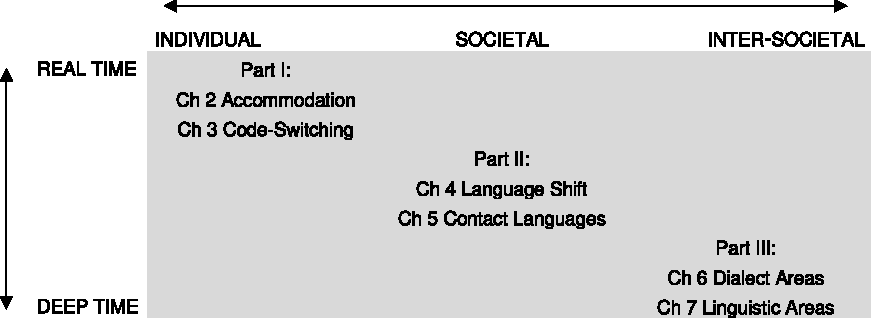
\includegraphics[width=1.0\textwidth]{Images/Structure1.pdf}
\label{figure1}
\end{figure}


In this book, based on a unified, recurring chapter structure,\footnote{\citet{adamouetal2021routledge} take the same approach, but this publication was not available to us at the time of conception of this book.} specialists of each of the subfields mentioned above give overviews of common practices in their respective fields, thus providing a platform for comparative contact linguistics. The remainder of this introduction is devoted to contextualizing and explaining the approach we take in this book. Section \ref{sec-connections} discusses a number of proposals for overarching frameworks for contact linguistics. These proposals highlight potential points of commonality between different contact phenomena, but at the same time, they each give a perspective on contact linguistics that is influenced by a particular subfield. In Section \ref{framework}, therefore, we propose an alternative approach. In this approach, we take a step back and look at the make-up of different research traditions within the general field of contact linguistics. In Section \ref{bridging}, we outline the key areas of synergy across the subfields and illustrate some of the most important overlaps among their approaches.

\section{Overarching frameworks for contact linguistics} \label{sec-connections}

 Several authors have proposed generalizations of language contact phenomena across the time scale and/or social scale. These studies form important pieces of the puzzle how the level of the individual in a real-time conversation connects to deep-time and society-wide historical changes due to contact. Without aiming for comprehensiveness, we discuss four illustrative models that highlight different factors in tying together contact phenomena.\footnote{These models were chosen because they are relatively recent, and because they contrast in terms of the factors and phenomena that they highlight. Older, highly influential models, like \citet{Weinreich1953Languages, thomasonetal1988language}, and \citet{van_coetsem_loan_1988}, are precursors of the models presented here, and as such, their conclusions have been incorporated into the more recent models in many ways.} However, they also make clear that, even if they have areas of overlap, these models regard contact effects from the perspective of a particular subdiscipline.
 

\subsection{\citet{niedzielskietal1996linguistic}: Language attitudes}
 
The first example is \textcite{niedzielskietal1996linguistic}, which is an attempt to apply the ideas and principles of Communication Accommodation Theory (CAT) to contact linguistics more broadly. CAT focuses on the relationship between language, social interaction, and social evaluation. According to CAT, speakers express social distance or social closeness to an interlocutor by becoming less or more similar in terms of their communicative behavior (divergence vs. convergence). For instance, speakers may start using the same linguistic expressions, adapt their speech rate to match the interlocutor's, or become more similar in their mimicry.
CAT was first developed and tested in social psychology, primarily out of an interest in person perception and the dynamics of conversation (for details, see Chapter \ref{chap_accommodation} on accommodation). 
Over the last decades, sociolinguists have become interested in the theory and used the model to explain linguistic patterns within a conversation (e.g. \citealt{coupland_accommodation_1984}).
 
\textcite{niedzielskietal1996linguistic} explicitly link phenomena of contact linguistics to CAT, suggesting several ways in which CAT can offer insights for longer-term contact effects. For instance, conversational research suggests that the extent to which L1 interference takes place is influenced by attitudinal factors \parencite{giles1979ethnicity}. A further application of CAT to contact linguistics discussed by \textcite{niedzielskietal1996linguistic} are creoles that have developed out of pidgins. According to this idea, creoles may be seen as varieties that arise as a result of repeated mutual accommodation in situations of maximal cultural-linguistic differences between communicating groups. CAT may also contribute to the understanding of how mixed (or intertwined) languages emerge, especially those that constitute secret codes. These varieties may come about as a result of conscious divergence from interlocutors of social out-groups. Finally, CAT can also generate insights on how dialect continua and linguistic areas develop. In areas with frequent contact between speakers of different dialects, dialect features may spread through convergence to speakers of another dialect if attitudinal factors are favorable and if speakers interact often enough. Accommodation research can shed light on the metalinguistic consciousness of specific parts of language, e.g. by investigating which linguistic parts are particularly prone to converge (or to be avoided) in interactions. From this point of view, accommodation research can improve our understanding of which linguistic elements are prone to be adopted by multilingual speakers, and therefore, which elements may spread in linguistic areas.\\

\subsection{\citet{matras&sakel2007}: Pivot matching and pattern borrowing}

The focus of \textcite{matras&sakel2007} is to identify the mechanism that is responsible for a particular type of contact-induced effect, where ``the patterns of distribution, of grammatical and semantic meaning, and of formal-syntactic arrangement at various levels (...) are modelled on an external source" (p. 829--830). In other words, this type of contact effect does not involve the transfer of form from one language to another, but more abstract organizational and functional principles. They call this type of contact-induced change \emph{pattern borrowing}.

\textcite{matras&sakel2007} propose what they call \emph{pivot matching} as the mechanism involved in pattern borrowing. They claim that bilinguals recognize a pivotal feature  of a construction in a model language and they replicate that in a functionally equivalent construction in the replica language. What the pivot of a construction is can only be established post-hoc: pivots are the elements of a construction that are copied from one language into the other (while using inherited material). \textcite{matras&sakel2007} present pivot matching as a creative process whereby bilingual speakers exploit their complete bilingual repertoire to create an utterance that is formally fully monolingual, but organizationally contains elements of both languages.

The reason for pivot matching to occur in the first place is, according to \textcite[832]{matras&sakel2007}, that bilingual speakers ``relax to some extent the need to distinguish
between their two repertoires when planning the utterance". Pivot matching is thus first and foremost an online discourse strategy. However, if the circumstances are favorable, these online strategies may lead to long-term effects, thus connecting conversational contact effects to contact-induced language change and linguistic areas. A requirement for pivot matching to have long-term effects is that the group of learners should be large enough, and the process of acquisition should never be complete. Furthermore, long-term effects of pivot matching are more likely to occur in societies with relatively lax norms when it comes to grammatical rules, so that pivot matching is not corrected.

Social constraints, for instance a social policy against mixing of language matter (phonetic substance), as e.g. in the Vaupés in Amazonia (see Chapter \ref{chap_areas}) may also facilitate or promote pivot matching, increasing the potential of long-term effects.


Matter borrowing (over pattern borrowing) may also be influenced by struc\-tur\-al-lin\-guis\-tic factors. These have to do with the resistance to or unlikelihood of matter borrowing for some highly entrenched linguistic elements such as inflectional morphology. More generally speaking, some constructions favor matter borrowing, others pattern borrowing, and yet others seem to have no clear preference. Linguistic constraints may also be relative, subject to the inventory of linguistic elements in the replica language that can be exploited for pivot matching in a particular construction. Other forces at work mentioned by \textcite{matras&sakel2007} are the fact that some features of constructions appear to be essential and thus immune to modification, and phonetic similarity.\\

\subsection{\citet{myersetal2009universal}: Lexicon versus structure}

A different overarching model is presented in \textcite{myersetal2009universal}. The central assumption of the model, which was originally developed to tackle certain types of code-switching phenomena, is that contact phenomena display non-random patterns in that they follow the \emph{structural patterns} of one language, inserting \emph{content} from other languages into this structural frame (the Uniform Structure Principle). The language that supplies the structure is referred to as the \emph{Matrix Language}, while the language that supplies content material that is inserted into the matrix is referred to as the \emph{Embedded Language}.

The second major part of the model is an elaboration of what is structure and what is content. Four types of morphemes\footnote{The term ``morpheme" is used in a generalized sense to refer to abstract entries or features and their surface realizations.} are distinguished: 


\begin{itemize}\sloppy
    \item{\textsc{Content morphemes}: conceptually salient material that receives or assigns thematic roles (i.e. argument roles such as agent, patient, beneficiary, etc.).}
    \item{\textsc{Early system morphemes}: conceptually salient building blocks of phrase structures, which do not receive or assign thematic roles (e.g. articles, derivational affixes, verbal particles).}
    \item{\textsc{Bridge late system morphemes}: Structurally assigned material that connects (builds bridges between) elements of a constituent and that depends on information within its constituent (e.g. markers of possession, partitive markers, expletives).}
    \item{\textsc{Outsider late system morphemes}: Structurally assigned material that depends on information outside of the immediate constituent (e.g. subject-verb agreement, case markers).}
\end{itemize}

The main idea is that the four morpheme types (content morphemes and the three system morpheme types) can be ordered as to how likely it is that they come from the embedded or matrix language in a mixed utterance (see \tabref{tab-ms-model}).

\begin{table}
\caption{Morpheme types and source languages\label{tab-ms-model}}  
 \resizebox{\textwidth}{!}{\begin{tabular}{lccr}
  \lsptoprule
 embedded language & & & matrix language\\ 
  \midrule
  content morphemes & early system morphemes & late bridges & late outsiders\\ 
   \lspbottomrule
 \end{tabular}}
\end{table}

The authors connect this to a psycholinguistic language production model proposed in \textcite{levelt1989speaking} in which, among other things, a distinction is made between selecting items (lemmas with associated forms) from a mental lexicon, and subsequently generating a grammatical context for these items.

Myers-Scotton \& Jake's claim is that content morphemes and early system morphemes are part of the mental lexicon, whereas late bridges and late outsiders are generated as part of the grammatical context. In this sense, their model stresses both linguistic structure and language processing as important factors in explaining contact patterns, at least in code-switching. 

According to \textcite[291]{myers1998way}, ``the same structural processes figure in all forms of bilingual speech, from code switching to interlanguage in second language acquisition, to language attrition, to mixed languages or pidgins and creoles". In other words, Myers-Scotton explicitly links individual, real-time behavior (code-switching) to historical processes at the societal level (language attrition, contact language formation), suggesting that they can be tackled by one and the same model (see e.g. \cite{myers1998way} for an elaboration).\\


\subsection{\citet{muysken2013language}: Social and linguistic asymmetries}

A framework for explaining language contact phenomena based on certain asymmetries between aspects of the first language (L1) and the second languages (L2) of a group of bilinguals is presented in \textcite{muysken2013language}. He introduces four general bilingual ``optimization strategies", which are typically applied by bilingual speakers in different sociolinguistic circumstances. These optimization strategies and their brief descriptions are given in \tabref{tab-muysken_OS}; the numbers are indices for later referral in the running text.

\begin{table}
\caption{Four bilingual optimization strategies}  
\label{tab-muysken_OS}
%\resizebox{\textwidth}{!}{
 \begin{tabular}{lll} 
  \lsptoprule
 No. & Shorthand & Description \\ 
  \midrule
  1 & L1 & Maximize structural coherence of the first language \\
  2 & L2 & Maximize structural coherence of the second language\\
  3 & L1/L2 & Match between L1 and L2 patterns where possible\\
  4 & UP & Rely on universal principles of language processing\\
   \lspbottomrule
 \end{tabular}
 %}
\end{table}

\textcite{muysken2013language} argues that these four generalized strategies are applied in different ways depending on the circumstances, leading to different outcomes, both in conversations and in patterns that are the result of sustained contact over time. Strategy 1 tends to occur in situations where L1 has high prestige and/or speakers of L1 have low proficiency in L2 and/or limited access to L2. Strategy 2 is often employed in opposite circumstances, i.e. where L2 has high prestige and/or proficiency in L2 is high and/or there are large numbers of L2 speakers. Strategy 3 is prototypically connected to situations of low normativity (i.e. where there is more social tolerance for using different structures), but also to situations where L1 and L2 are lexically and/or typologically similar to each other. The final strategy 4 is found in situations where the social and linguistic distance between the L1 and L2 groups is large and/or the contact period brief.

Muysken's model is best illustrated by looking at code-switching, for which it seems to be developed in most detail. Based on earlier work \parencite{muysken2000}, he distinguishes four different patterns in code switching (\tabref{tab-muysken_CS}).

\begin{table}
\caption{Four bilingual optimization strategies\label{tab-muysken_CS}}  
 \begin{tabularx}{\textwidth}{lX} 
  \lsptoprule
 Type & Description \\ 
  \midrule
  {Insertion} & One of the languages (L1) is used as the matrix language, and the other (L2) as the embedded one.\\
  {Congruent lexicalization} & Elements from either language are used in constructions that are (partly) shared by the languages.\\
  {Alternation} & Fragments of L1 and L2 are used in succession within a sentence, regulated by universal combinatory possibilities.\\
  {Backflagging} & Material from the heritage language (L1) is inserted in an otherwise L2 discourse.\\
\lspbottomrule
 \end{tabularx}
\end{table}

Muysken connects each of these strategies to one of the optimization strategies mentioned in \tabref{tab-muysken_OS}. Insertion is considered to be the result of strategy L1, because it inserts content elements from L2 in an otherwise L1 structural environment. As such, the structural coherence of L1 is maximized (kept intact). Congruent lexicalization results from the L1/L2 strategy, in that it is an attempt to combine elements from both languages that are partly shared. Alternation can be connected to the strategy UP to the extent that the way in which elements from both languages are combined follows universal principles. Backflagging, finally, results from the L2 strategy, because the structural integrity of L2 is respected, and elements of the heritage language are inserted. This is the mirror image of insertion.

\textcite{muysken2013language} explicitly claims that these strategies are responsible for many different contact phenomena at different social scales and time depths. It is beyond the scope of this introduction to discuss this in detail (the reader is referred to \cite{muysken2013language} for this), but the model and its interpretations for other contact phenomena relevant to this book are given in \tabref{tab-muysken}.

\begin{table}
\caption{Bilingual optimization strategies and contact phenomena}  
\label{tab-muysken}
%\resizebox{\textwidth}{!}{
 \begin{tabularx}{\textwidth}{l QQQ} 
  \lsptoprule
 & Code-switching & Contact languages & Contact-induced change \\ 
  \midrule
  L1 & insertion & relexified languages, L1-oriented pidgins & borrowed forms adapt to L1 functionality 
  
  \\
  
  L2 & backflagging & lexifier-oriented contact languages  & transfer, substrate\\
  &&&
  
  \\
  
  L1/L2 & congruent lexicalization & compromise contact languages & merging aspects from both languages, convergence
  
  \\
  
  UP & alternation & bioprogram & simplification, adopting unmarked structures\\
   \lspbottomrule
 \end{tabularx}
 %}
\end{table}

Of relevance to the present book is that Muysken identifies a set of factors that are involved in the choice of optimization strategy \parencite[726]{muysken2013language}. We come back to the issue of factors in the next section and at various points in the book.

\begin{itemize}
\item similarity factors (lexical and typological);
\item prestige and status factors;
\item proficiency factors;
\item contact factors (group size, network type);
\item time factors (of contact period);
\item attitudinal factors (low normativity, political distance).
\end{itemize}

\subsection{Comparing models}
What the models described above have in common is that they point to phenomena that recur in different contact-related situations, from language-mixing patterns in real-time bilingual conversations to deep-time contact effects that have spread through entire communities. They differ in what they see as crucial factors contributing to these recurring patterns. Where Niedzielski
and Giles \parencite*{niedzielskietal1996linguistic} highlight the importance of attitudinal factors, Matras and Sakel \parencite*{matras&sakel2007} focus on language processing, Myers-Scotton and Jake's \parencite*{myersetal2009universal} model gives central stage to linguistic structure and the lexicon-structure distinction, and Muysken's model focuses on optimal communication strategies of bilinguals given certain (a)symmetries in the circumstances (taking into account aspects such as language access, power relations, and typological distance).

These models suggest that contact phenomena from individual conversations to Sprachbund phenomena are connected, but they also highlight that several perspectives on the factors contributing to these connections are possible. This makes it hard to bring all these different perspectives together. One of the reasons for the different focal points may be that the authors in the models presented above look at different contact effects through a particular prism (whether that is an accommodation prism, a code-switching prism, a convergence prism, or a symmetry prism). 

\section{The approach of the present book} \label{framework}

The present book differs from these (and other) approaches in two main respects. First, it is a multi-authored effort that involves specialists from the different subdisciplines that are central to this book. This ensures an even-handed treatment of each subdiscipline. Second, rather than focusing only on what the implications of the results of subdiscipline A are for subdiscipline B, it takes a further step back and compares the research traditions of each subdiscipline. 

While \figref{fig-structure1} suggests that the phenomena described in the book are maximally different from each other, a more detailed overview reveals that each of the subfields addressed has a broader range and overlaps with neighboring fields, as shown in \figref{fig-structure2}, where numbers between brackets refer to chapters.

\begin{figure}
\caption{The relationship between each of the book's topics with the two dimensions, time and social scale} \label{fig-structure2}
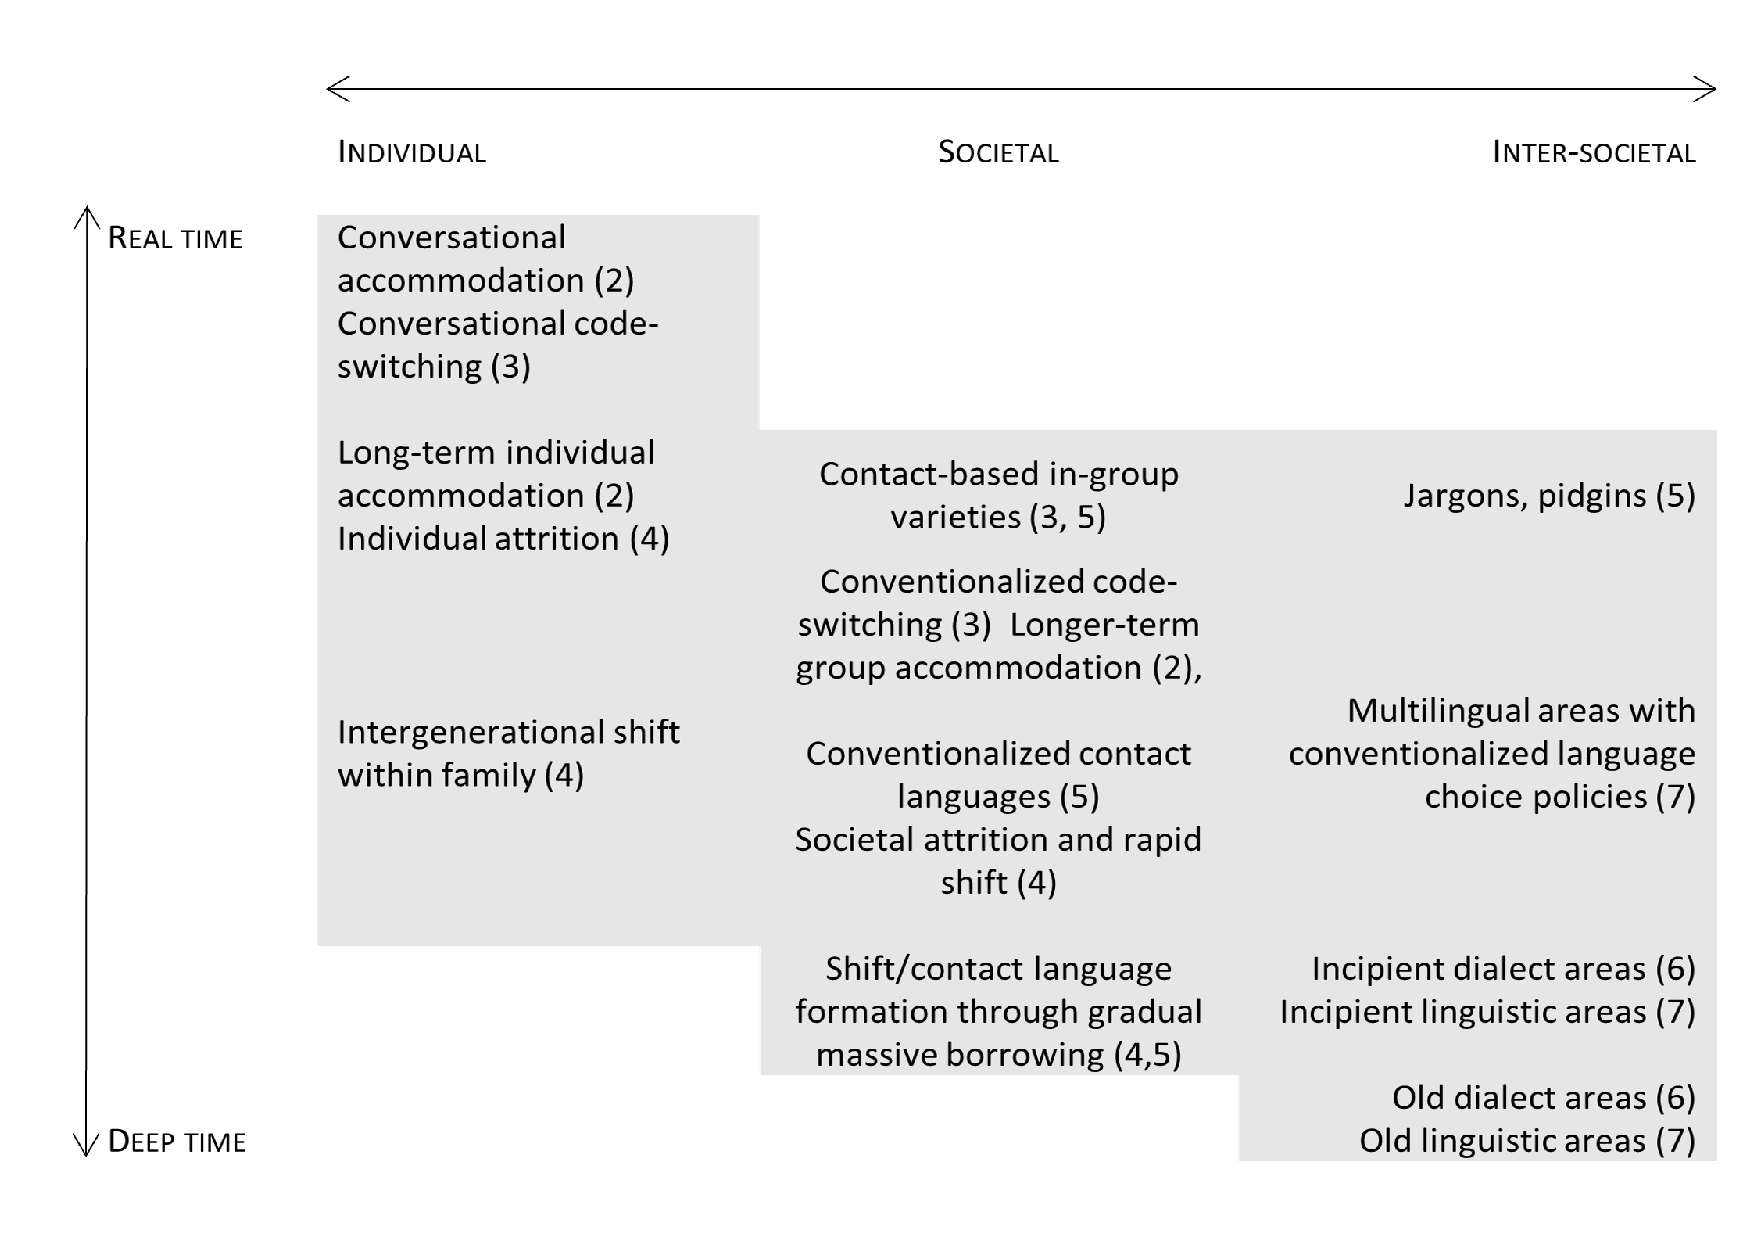
\includegraphics[width=1.0\textwidth]{Images/Structure2.pdf}
\label{figure2}
\end{figure}

These overlaps allow for more in-depth comparisons between different phenomena across the subfields and for a more precise assessment of the effects of time, social scale, and of course research practices.

\subsection{Approaches}
In the sections entitled Approaches all authors present the ways in which their subfield models its predictions on the basis of empirically available data. This is done explicitly to illustrate the potential for comparison across subfields. Studies concerned with conversational interactions model the effects of short-term contact-induced effects into deeper time, predicting how conversational patterns may lead to contact-induced change (see in particular \cite{niedzielskietal1996linguistic} on how patterns of accommodation in conversations may lead to patterns of convergence, or \cite{myers2008language} on how patterns found in conversational code switching recur in all products of language contact). Areal studies often only have the present-day linguistic patterns at their disposal, and therefore their models seek to reconstruct the past scenario(s) that gave rise to the present situation \parencite[see e.g.][]{muysken2010scenarios, Nichols2003Diversity}. Modeling in the study of contact varieties and language shift may go both ways: predicting what scenarios will lead to contact varieties or language shift, or filling the gaps of the often incomplete historical record on the basis of synchronic (language) data.

Therefore, a comparison of models and empirical evidence across subfields can be mutually beneficial: interactional research can test their predictions by looking at areal patterns and patterns in contact varieties and language loss, and the study of contact varieties, language shift, and areal linguistics can be informed by accommodation or code-switching studies about possible outcomes of individual interactions.


\subsection{Linguistic patterns}
All of the subfields discussed in this book are invested in the question ``What type of linguistic patterns do we observe?" Because all approaches try to generalize across the different patterns found for the particular phenomenon in question (code-switching patterns, typical creole structure, features prone to diffuse, etc.) they form a basis for direct comparison: to what extent do we find similar patterns in, for instance, code-switching and mixed languages, in contact dialectology and linguistic areas, and in accommodation and language shift? In some subfields of contact linguistics, the linguistic patterns are typically discussed together with the processes that give rise to them. Therefore, three chapters in this book introduce these processes in conjunction with the patterns.


\subsection{Factors}
Last, all chapters discuss factors that may influence the observed outcomes. Some of these factors relate to characteristics of individuals (e.g. age, attitudes) or the speech situation (e.g. conversational topic), while others relate to the varieties involved (e.g. typological distance), to societal parameters (e.g. subsistence strategies, language ideologies), or to the geographical circumstances (e.g. topographical elements that facilitate or impede contact, travel distance). Despite the fact that conversational approaches put more emphasis on characteristics of the individual and the speech situation, and areal approaches on geographical factors, there is an overlap in particular in the societal and linguistic factors involved, allowing for a relatively direct comparison.

\section{Bridging the gap} \label{bridging}

With this book, we argue that seemingly disparate contact phenomena can be connected by making reference to two dimensions: time and social scale. The maximum contrast spelled out by these dimensions is, on the one hand, between the real-time effects in multilingual conversations as studied by code-switching and accommodation studies, and, on the other hand, the deep-time effects observable in sizable linguistic areas. It goes without saying that contact linguistics operates on many more dimensions than social scale and time depth alone, and in this respect we do not aim for completeness. However, we do want to highlight some further dimensions that play a role in this book, and which for their part allow for other connections between subfields.

An obvious opposition between dialect areas and linguistic areas is genealogical relatedness (which is usually associated with typological similarity). This opposition partly recurs in the opposition between accommodation and code-switching, phenomena that are usually observed between closely related and unrelated or only distantly related languages, respectively.

A second opposition worth mentioning is between contact-induced language birth and language death, Chapters \ref{chap_shift} and \ref{chap_contactlanguages} of this book, respectively. There may be many sociolinguistic processes giving rise to the formation of linguistic areas, including language shift, societal L2 effects, and language mixing, all of which are discussed in the chapters on language shift and contact varieties. The opposition birth vs.death of varieties, finally, may be the societal outcome of accommodation or code-switching.

As a result of the differences in the time-depth and the social scale of the contact phenomena, all subfields deal with varying levels of opacity regarding the linguistic components and their origin. For instance, a loanword that initially entered a language as a recurring element of another language is bound to gradually lose its identifiability as a foreign word as it becomes integrated into the sound system. It is then no longer marked by restricted grammatical and pragmatic contexts, and the semantics that point to an outsider culture become bleached over time. In code-switching (CS) studies, the linguistic elements are evaluated on a CS – borrowing continuum, and this has led to numerous attempts to define and clarify these concepts. At the other end of the scale, in the study of linguistic areas, even the donor language of a feature may remain unknown while its contact-induced origin may be obvious. Overcoming these ambiguities has led to several methodological improvements in the field.

However, opacity does not result from the time and social scale alone. It emer\-ges from the chapters of this book that in describing, explaining, and modeling language contact all fields deal with three major confounding dimensions: variation, diffusion, and universals. Yet the emphases and thus often implicit understanding of these vary from subfield to subfield.

\textit{Variation}, especially conditioned by sociolinguistic factors, is at the center of most models and approaches presented in this book. The chapters on accommodation and CS are excellent reminders of the fact that conversational contact phenomena are highly indexical, which may explain why the long-term outcomes of these phenomena are so hard to predict. On the other hand, the chapters on language shift and new languages introduce detailed models on the sociolinguistic factors contributing to community-level phenomena due to the abundance of recent or even real-time cases to be observed. Finally, a more fine-grained understanding of sociolinguistic variation has led to advances in the study of linguistic and contact dialectology, although tying specific sociolinguistic settings to specific types of variables of language change remains one of the most debated issues.

\textit{Diffusion} forms a significant explanandum in all approaches that deal with at least community-size phenomena. Contact-induced language change is initiated in recurring multilingual interactions. Yet, the areal distribution of contact-induced features within linguistic areas shows that monolingual communication must often be the main channel of their propagation, as these phenomena are also evidenced in historically monolingual areas. Here, the observations regarding closely related varieties in interaction are invaluable in understanding the pathways of the diffusion of innovations.

\textit{Universals} play different roles in evaluating contact phenomena, depending on the field. The role of universals in the emergence of contact varieties is among the big questions of linguistics of the past decades. In CS studies, universal principles are a built-in factor in some models, but the field has also produced certain robust predictions claimed to hold universally. In the study of linguistic areas, typological universals are an important indicator in deciding the weight of a feature as evidence for a contact area, since implicational typological universals may offer an alternative explanation to an areal bundling of linguistic features.

It is exactly this type of overlap in patterns, factors, and dimensions across fields of contact linguistics that inspired this book. We hope that the following chapters offer the reader similar moments of discovery and illumination as they have for the authors.

%\section*{Abbreviations}
\section*{Acknowledgements}

We thank all the participants of the first (post)doc retreat in 2014 in Wangs, St. Gallen, and Giorgio Iemmolo for originally bringing up the idea of connecting aficionad@s of dialect and language contact. We thank all the participants of subsequent discussion sessions at the University of Zurich, and those of the second postdoc retreat in 2017 in Filzbach, Glarus, for fruitful discussions, writing, and taking this book project further.

URPP (University Research Priority Program) Language and Space and ZüKL (Zürcher Kompetenzzentrum Linguistik, now LiZZ, Linguistik Zentrum Zürich) at the University of Zurich financially and logistically supported the retreats and the genesis of this book. 

Rik van Gijn gratefully acknowledges the support of the European Research Council (ERC) under the European Union’s Horizon 2020 research and innovation programme (grant agreement No. 818854 - SAPPHIRE). Max Wahlström wishes to acknowledge that his embarking on this book project was only possible due to the support of the Kone Foundation.



\printbibliography[heading=subbibliography,notkeyword=this]
\end{document}
